\documentclass[onecolumn,11pts]{IEEEtran}
\usepackage[utf8]{inputenc}
\usepackage{listings}
\usepackage{xcolor}
\usepackage{url}
\usepackage{hyperref}
\usepackage{graphicx}
\usepackage{anysize}
\usepackage[spanish]{babel} 
\usepackage[utf8]{inputenc} 
\usepackage{multirow}
\marginsize{3.5cm}{2.5cm}{3cm}{3cm} 
\hypersetup{
  colorlinks=false,       % false: boxed links; true: colored links
  pdfborder={0 0 0}       % remove ugly border from links
}


\markboth{Redes de Datos}%
{Informe}
\date{Junio 2017}

\begin{document}

\begin{titlepage}

\begin{center}
\vspace*{-1in}
\begin{figure}[htb]
\begin{center}

\includegraphics[scale=0.4]{logo_udp}
\end{center}
\end{figure}
Facultad de Ingeniería y Ciencias\\Escuela de Informática y Telecomunicaciones\\
\vspace*{0.15in}
\vspace*{1in}

\begin{LARGE}
\textbf{Laboratorio N6: Redes de Datos\\
'Sockets'} \\
\end{LARGE}
\vspace*{1in}
\begin{large}
Profesor: José Pérez \\Ayudante: Alexis Inzunza \\ Fecha: 09-06-2017
\end{large}
\vspace*{0.3in}
\vspace*{1in}
\begin{large}
\begin{flushright}

Integrantes: \\
Benjamín Alvarez \\ Nicolás Reyes \\ 
\end{flushright}
\end{large}
\end{center}
\end{titlepage}


\tableofcontents % indice de contenidos

\cleardoublepage

\cleardoublepage
\listoffigures
\title{Actividades de Laboratorio}

\maketitle
    El objetivo de este laboratorio es crear un algoritmo simple de cliente y servidor para un chat usando sockets, pero primero, ¿Qué es un socket?
    Un socket es un organismo que permite el intercambio de información entre un cliente y un servidor. Para poder usarlo necesitaremos ciertas herramientas.
    Estás serán los identificadores o IP's de dos computadores, un protocolo de transporte (TCP o UDP) y dos números de puerto, uno local y otro remoto. En este caso usaremos el protocolo TCP ya que este ofrece muchas mas confiabilidad cuando mandamos un mensaje, y es lo que generelamente se busca tener en un chat, ya que este debe ser entre dos personas o más pero no salir de ese grupo de conversación.\\
\section{Actividad 1}
    Para crear el cliente y el servidor usaremos el lenguaje de programación Python por un tema de comodidad. También haremos uso de API conocida como "Sockets de Berkeley":
        
   \begin{figure}[h!]
\centering
 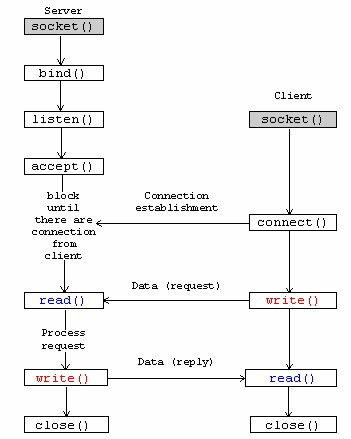
\includegraphics[scale=0.7]{image007}
\caption{Sockets de Berkeley}
\label{fig:image007}
\end{figure}
\newpage
    Las funciones que se utilizarán son las siguientes: 
    \begin{itemize}
    \item socket.socket([family[, type[, proto]]]): Es el constructor del socket y sirve para instanciarlo. En este caso vamos a usar sockets de internet, por lo que el primer parámetro será socket.AF\_INET y el segundo dependerá del protocolo que usemos, si es UDP se usa socket.SOCK\_DGRAM y para TCP será socket.SOCK\_STREAM.
    \item socket.bind(address): Este recibe una tupla que contiene el string de la IP host y el int del puerto a usar en nuestro servidor.
    \item socket.listen(backlog): Deja a nuestro server escuchando por conexiones. El parámetro que usemos dependerá de cuantas conexiones queremos mantener en cola, por ejemplo si ponemos 5 el servidor esperará a tener 5 conexiones para aceptarlas a todas. En general el número usado es 1.
    \item socket.accept(): Acepta una conexión. Retorna un socket y su address, que corresponde a la información del cliente.
    \item socket.recv(bufsize[, flags]): Se utiliza para recibir los datos del cliente. El bufsize indica la cantidad de bytes máximo admitidos, en general se usa 1024.
    \item socket.send(string[, flags]): Lo utiizaremos para enviar los datos. El parámetro que enviaremos es un string.
    \item socket.close(): Cierra el socket. Se utiliza una vez se termina el intercambio de información.\\
\end{itemize}

\\Ahora que conocemos las funciones empezaremos a crear el cliente. Lo primero que debemos hacer tanto en el cliente como en el servidor es importar socket escribiendo 'import socket' al principio de nuestro código.\\Después definimos el host y el puerto a usar, en este caso el host será la IP de Loopback y el puerto será 5000. Después de eso crearemos nuestro socket usando la primera función nombrada anteriormente, entregandole los parámetros socket.AF\_INET y socket.SOCK\_STREAM, el segundo es porque trabajaremos con TCP.\\Luego de tener creado nuestro socket usaremos la función socket.connect() y le pasaremos el host y el puerto en una tupla. Ahora pediremos en mensaje que se va a enviar con raw\_input y lo enviamos con socket.send(1024), luego cerraremos el client con socket.close(). El código quedará de esta forma:

\begin{figure}[h!]
\centering
 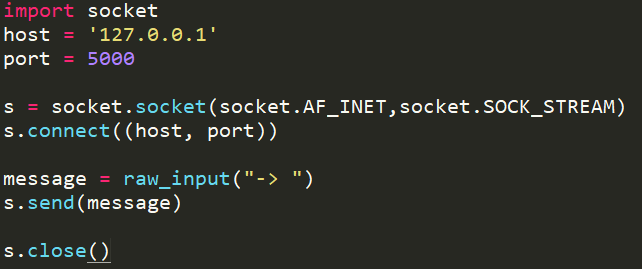
\includegraphics[scale=0.5]{cliente}
\caption{Cliente}
\label{fig:cliente}
\end{figure}

Ahora crearemos nuestro servidor:\\
Nuevamente al principio escribiremos 'import socket' y definiremos nuestra IP host y el puerto, que debe ser el mismo que pongamos en nuestro cliente. Con eso listo usaremos la función socket.bind() para bindear el host y el puerto a nuestro servidor. Luego usaremos socket.listen para empezar a aceptar conexiones, en este caso el parámetro que le pasaremos será 1. Despúes usaremos socket.accept() para recibir el socket del cliente y su información, esta información la imprimiremos en el servidor. Por último recibiremos el mensaje del cliente usando socket.recv(1024) y también lo imprimiremos. Por último usaremos socket.close() para cerrar nuestro servidor. El código debería quedar así:

\begin{figure}[h!]
\centering
 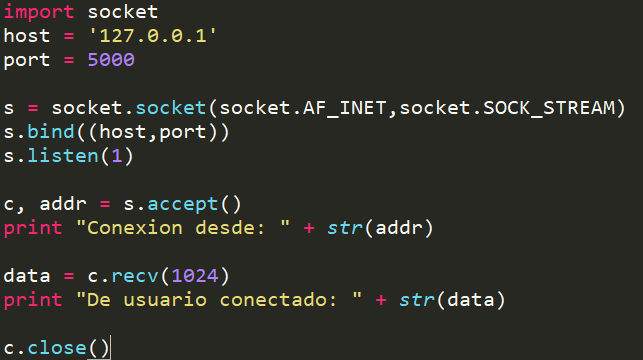
\includegraphics[scale=0.5]{server}
\caption{Servidor}
\label{fig:server}
\end{figure}
\newpage
\section{Actividad 2}
Utilizamos Wireshark para ver que sucedía al ejecutar nuestro programa y los resultados fueron los siguientes: 
\begin{figure}[h!]
\centering
 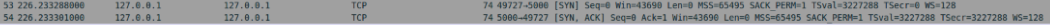
\includegraphics[scale=0.55]{ws1}
\caption{Wireshark conectarse el cliente al servidor}
\label{fig:ws1}
\end{figure}
\begin{figure}[h!]
\centering
 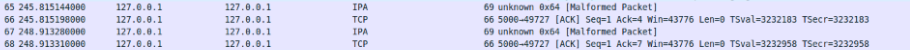
\includegraphics[scale=0.55]{ws2}
\caption{Wireshark al enviar mensajes desde el cliente}
\label{fig:ws2}
\end{figure}
\begin{figure}[h!]
\centering
 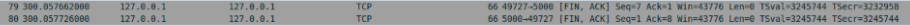
\includegraphics[scale=0.55]{ws3}
\caption{Wireshark cuando el cliente se desconecta}
\label{fig:ws3}
\end{figure}

\newpage
\section{Análisis y preguntas}
\begin{enumerate}
\item Utilizando la información obtenida en la actividad 2, explique el funcionamiento del envío y recepción
de información para su algoritmo, respondiendo a las interrogantes ¿Qué se envía? ¿Cómo se envía?\\
R: Como el protocolo que usamos es TCP, lo que se envia no es solamente el puerto de origen y de destino más el mensaje, sinó que se envian una serie de verificaciones para comprobar que el mensaje llegue correctamente a su destino.
\item ¿Por qué el puerto que muestra el servidor al generar la conexión no es el mismo que el escrito en el
algoritmo del ciente?\\
R: Esto es porque el cliente generalmente usa un puerto aletorio para conectarse a un servidor con un puerto específico. El servidor responde usando este puerto aleatorio. Por lo tanto el cliente y el servidor no están en el mismo puerto.

\item Si usted tuviese que realizar un videojuego con soporte multijugador utilizando sockets ¿Qué protocolo
utilizaría? ¿Por qué?\\
R:Si hablamos de un multijugador masivo el protocolo que se usa generalmente es UDP, ya que este aunque no asegura la llegada del paquete si asegura mucha rápidez y en juegos donde hay 64 personas al mismo tiempo la rápidez es necesaria. En otros juegos como por ejemplo los de cartas online que son entre dos personas creo que el mejor protocolo sería TCP ya que no se necesita rápidez, sinó lo que se necesita es mandar bastante información y asegurarse de que este llegue a su destino.
\item ¿Se puede utilizar cualquier número de puerto para cualquier aplicación? Explique.\\
R: No, los puertos que se pueden utilizar pueden ir desde 1024 hasta 49151. Esto es porque los puertos inferiores a 1024 son de uso exclusivo del sistema operativo, y los mayores de 48151 hasta 65535 son para uso privado y no pueden ser usados por cualquier aplicación.

\end{enumerate}
\newpage





\newpage
\section{Conclusión}
En esta actividad aprendimos como crear un cliente y un servidor para un chat, usando el protocolo TCP y además como se envia este mensaje. También pudimos conocer la diferencia entre los protocolos TCP y UDP y revisar cual es el que serviría mas en distintas situaciones. También conocimos los puertos que se pueden o no usar para crear estos servidores. Por último conocimos los socket y sus funciones y como operan.


\clearpage

\begin{thebibliography}{15}

\bibitem{mfp}
  omicrono,
  \emph{¿Por qué una partida online ocupa menos ancho de banda que una página web? }
  \url{http://omicrono.elespanol.com/2016/09/videojuego-online-tiempo-de-carga/}
  \bibitem{mfp}
  superuser,
  \emph{Is the same port acting as both client and server?}
  \url{https://superuser.com/questions/683965/is-the-same-port-acting-as-both-client-and-server}

\end{thebibliography}

\end{document}